
%%%%%%%%%%%%%%%%%%%%%%%%%%%%%%%% 
\section{The Time Projection Chamber (TPC)} 
\label{sec:detectors-fd-ref-tpc}

\subsection{Overview}

The scope of the Time Projection Chamber (TPC) subsystem includes the design, procurement, fabrication, testing, delivery of  anode plane assemblies (APAs),  cathode plane assemblies (CPAs), field cage, and feedthroughs, filtering networks, cables and power supplies for the cathode high voltage system.

The requirements for the TPC can be found in the requirements documentation \cite{lar-fd-req}. The most significant ones are the following. The TPC must:

\begin{itemize}	
\item Meet the physics requirement for electron/photon discrimination;  the TPC wire spacing will be $<$~5~mm
\item Limit variation in the wire sag to $<$ 0.5~mm such that it does not significantly impact the position and energy resolution of the detector
\item Provide redundancy in the discrimination of electrons from photon conversions and ensure long-term reliability over the life of the experiment;  configuration will use three instrumented wire planes
\item Optimize the measurement of high-energy and low-energy tracks from accelerator-neutrino interactions; the wire-plane orientation is optimized for neutrinos in the DUNE energy range
\item Use only materials that are compatible with high-purity liquid argon
\end{itemize}

The Time Projection Chamber is the active detector element of LAr-FD. It is located inside the cryostat 
vessel and is completely submerged in liquid argon at 89~K. The TPC consists of alternating anode plane 
assemblies (APAs) and cathode plane assemblies (CPAs), with field-cage modules enclosing the four open sides between the anode and cathode planes.
When proper bias voltages are applied to the APAs and CPAs, a uniform electric field is created in volume between the anode and cathode planes. A charged particle traversing this volume leaves a trail of 
ionization in the ultra-pure liquid argon.  The electrons drift toward the anode wire planes, inducing electric current signals in the front-end electronic circuits connected to the sensing wires.  The current 
signal waveforms from all sensing wires are amplified and digitized by the front-end electronics, and transmitted through cold cables and feedthroughs to the data acquisition system outside of the cryostat.


\begin{cdrfigure}[Cross section of the TPC inside the cryostat]{tpc-xsect1}{Cross sections of the LBNE 5 kton TPC (left) vs. the DUNE 10 kton TPC (right).  The exchange of the APA and CPA positions significantly reduced the energy stored in the TPC by eliminating the two ground facing cathode planes. This allows an increase in the detector's fiducial volume with the same cryostat.  The length of the DUNE TPC is  58~m along the direction of the neutrino beam (into the paper)}
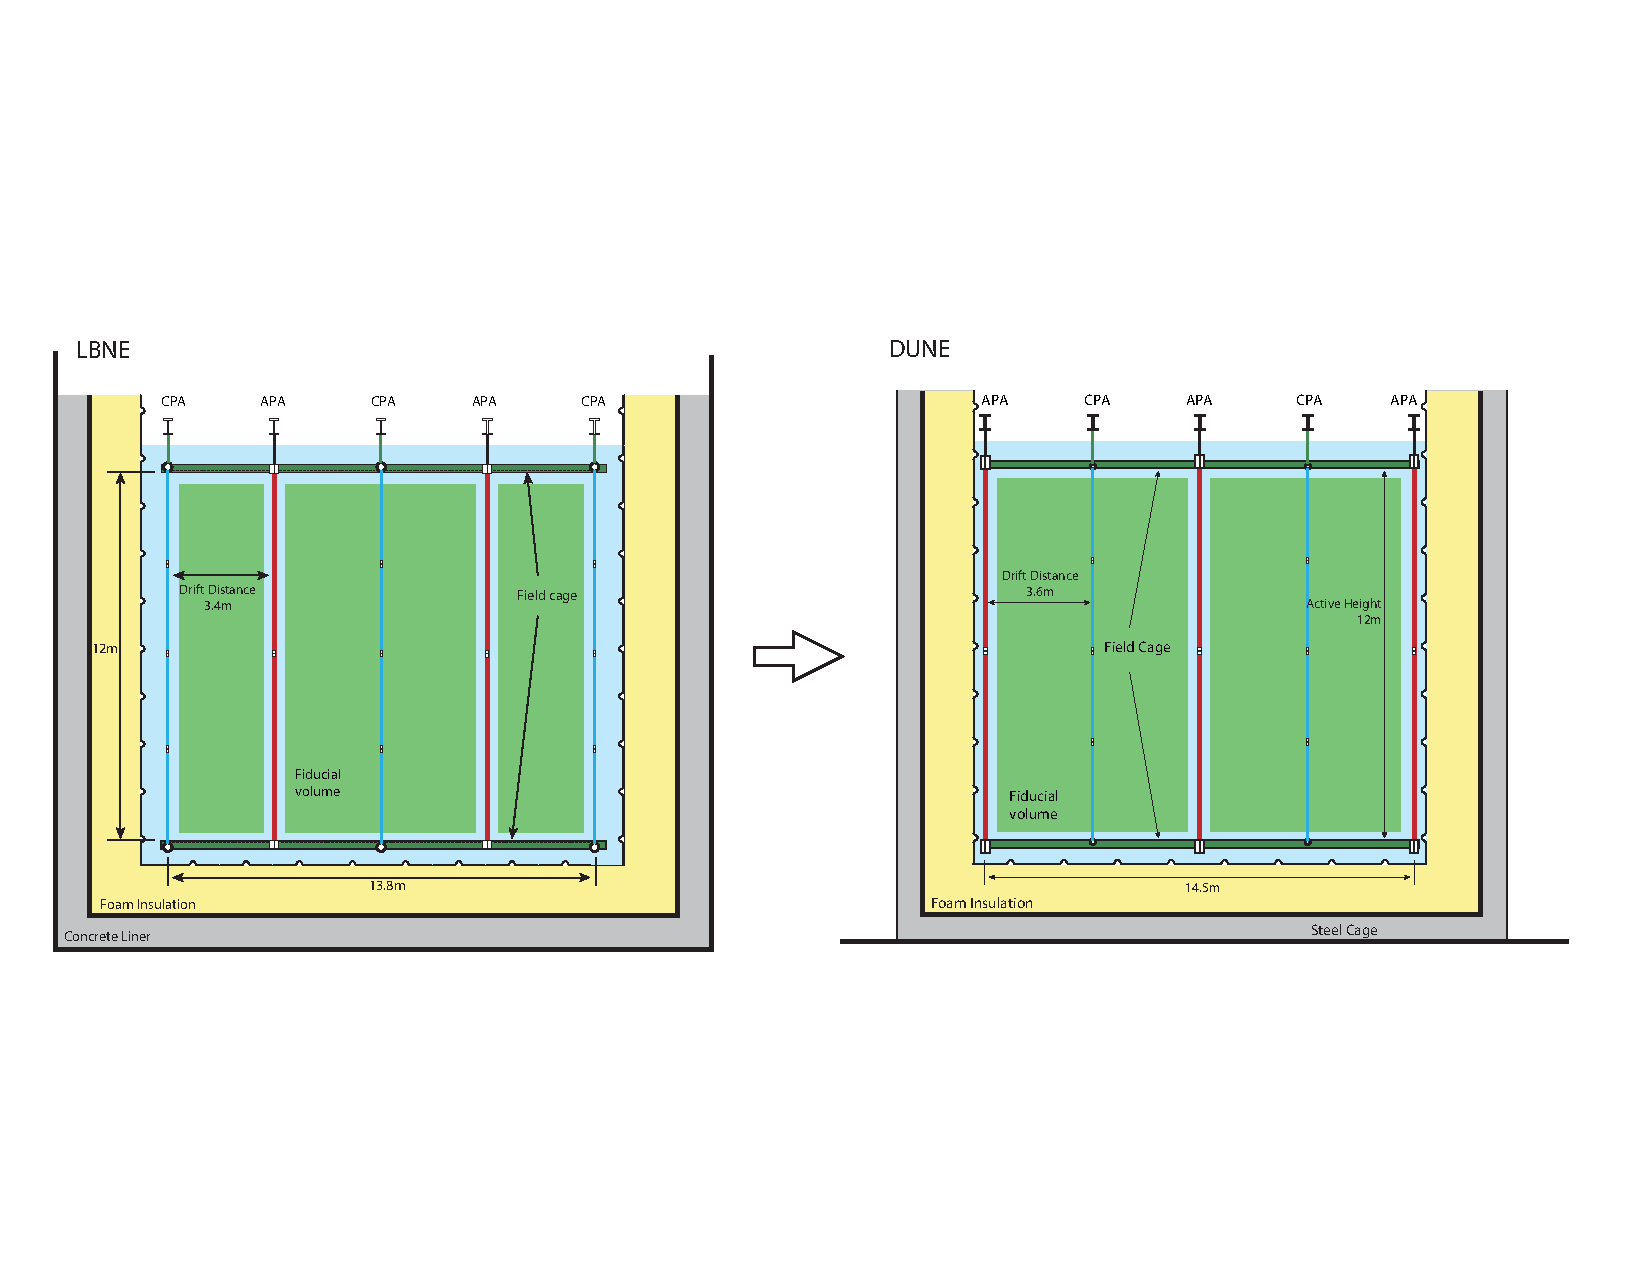
\includegraphics[width=\linewidth]{tpc_xsection_lbne_dune.pdf}
\end{cdrfigure}


The TPC's active volume (Figure~\ref{fig:tpc-xsect1}) is 12~m high, 14.5~m wide and 58~m long in the beam direction. 
Its three rows of APA planes interleaved with two rows of CPA planes 
are oriented vertically, with the planes parallel to the beamline. The  
electric field is applied perpendicular to the planes.
The maximum electron-drift distance between a cathode and an adjacent 
anode is 3.6~m. This requires a $-$180~kV bias voltage on the cathode plane to reach the 500~V/cm nominal drift field. The anode plane assemblies are 
2.3~m wide and 6~m high. Two 6~m modules stack vertically to 
instrument the 12~m active depth. In each row, 25 such stacks are placed edge-to-edge 
along the beam direction, forming the 58~m active length of the detector.  Each CPA has the same width, but half the height ($\sim$3~m) as an APA, for ease of assembly and transportation.  Four CPAs will be stacked vertically to form the full 12~m active height. 
Each cryostat houses a total of 150~APAs and 200~CPAs.
Each facing pair of cathode and anode rows is surrounded by a 
``field cage,'' assembled from panels of FR-4 sheets with parallel copper strips connected to resistive divider networks. 
The entire TPC is suspended through 5 mounting rails under the cryostat ceiling (see Figure~\ref{fig:tpc-floor-view}).


\begin{cdrfigure}[A view of the partial assembled TPC]{tpc-floor-view}{A view of the partially installed TPC inside the membrane cryostat.  The APAs are shown in red, CPAs are in cyan, field cage modules in yellow/green. Some of the field cage modules are in their folded position against the cathode.}
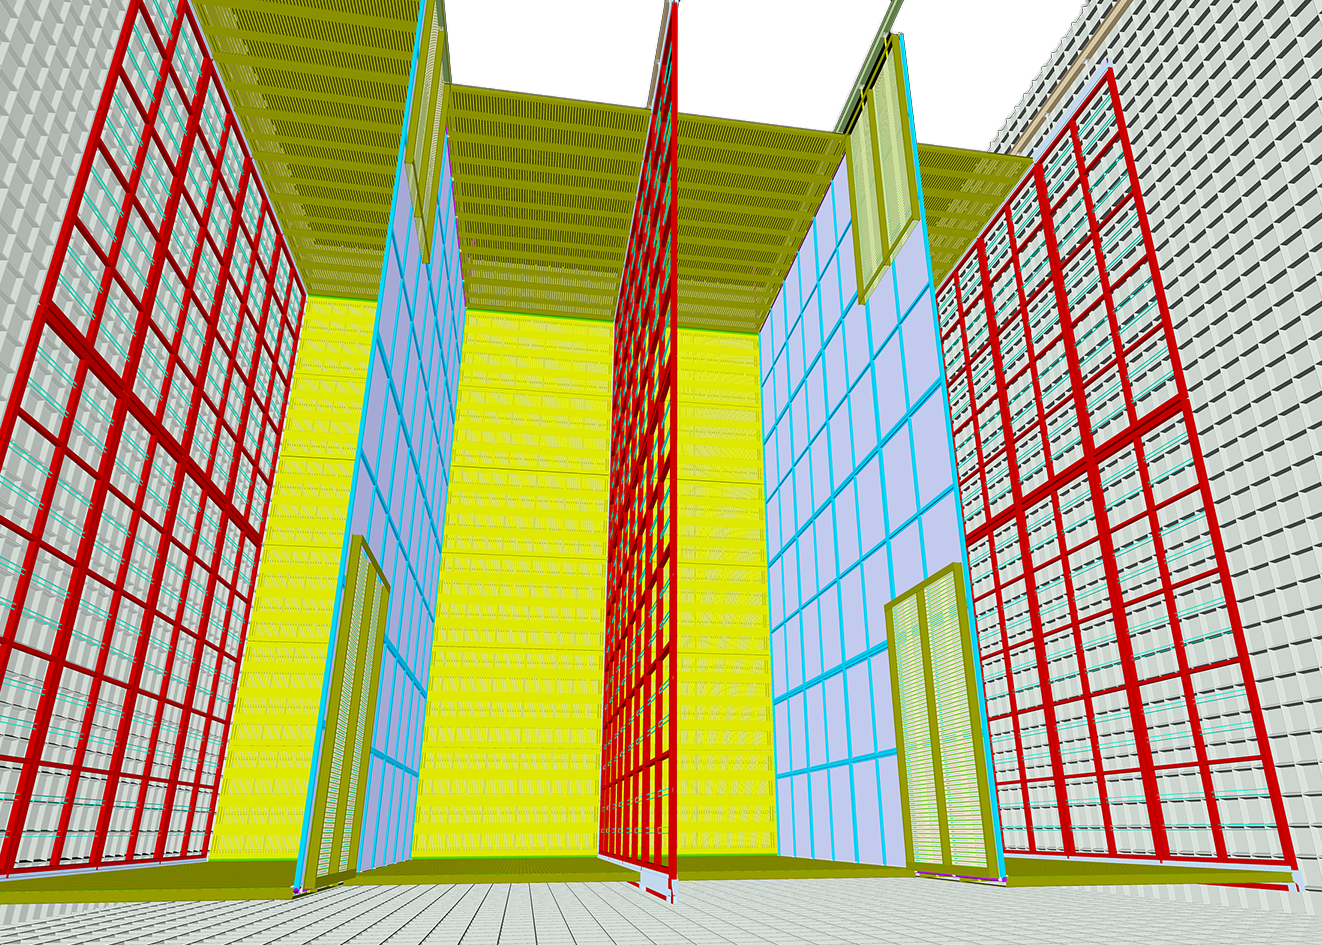
\includegraphics[width=\linewidth]{tpc_floor_view.png}
\end{cdrfigure}

The units of construction of the active detector are the APAs, CPAs, and field cage modules. These are modular elements of a size optimized
so as to simplify the manufacture, satisfy the commercial highway and underground transport requirements,
and facilitate handling and the speedy installation in the cryostat.  Each element will be fully tested in LN$_2$ (or LAr) after manufacture site,
again at the far detector site before installation, and finally will be monitored continuously during and
after installation to detect any failures due to damage occurring throughout the duration
of the installation operation. 


%%%%%%%%%%%%%%%%%%%%%%%%%%%%%%%% 
\subsection{Anode Plane Assemblies}
\label{subsec:fd-ref-apa}

The APAs are 2.3~m wide, 6.3~m long, and 12~cm thick. The length is chosen for fabrication purposes and compatibility with underground transport limitations. The 2.3~m width is set to fit in a standard HiCube container for storage and transport with sufficient shock absorbers and clearances. 
Each APA is constructed from a framework of light-weight, stainless-steel rectangular tubing, with four layers of wires wrapped over both sides of the frame. The front-end electronics boards are mounted on one end of the wire frame and protected by a metal enclosure.  


%%%%%%%%%%%%%%%%  
\subsubsection{Wire Planes}
\label{subsec:fd-ref-wireplanes}

150\,$\mu$m copper beryllium (CuBe) alloy wire is used on the APAs for its high break load, good electrical conductivity, excellent solder-ability and its thermal-expansion coefficient compatible to that of the stainless-steel frame.  The wires will be epoxied to fiberglass wire bonding boards and then soldered to copper traces on the boards for electrical connections.

On each APA, four planes of wires cover each side of a frame (the ``wire frame''); see Figure~\ref{fig:tpc-wire-frame-xsect}.
These four planes of wires are labeled, in order from the outside in: G (for grid), U, V and X.  
Table~\ref{tab:wire-parameters} summaries the key parameters of each of the wire planes.  The distance between wire planes is set to 4.76\,mm.  Each wire plane is biased to a particular voltage such that the ionization electrons from charged particle tracks will drift pass the first 3 wire planes and completely collected by the last (X) wire plane.  The V wires are DC-coupled to the readout electronics to minimize the maximum voltage on the other wire planes.
A grounded mesh plane with good optical transparency, located 4.8~mm behind the collection plane, prevents the electric field around this set of wires from being distorted by the metal frame structure and the wires on the opposite side of the frame. It also shields the sensing wires from potential EM interferences from the silicon photomultipliers (SiPMs) on the photon detectors, mounted within the frame.  
Each wire on the U,V and X planes is connected to a front-end readout channel. The Grid plane wires are not read out, but serve the important purpose of shielding the U wires from responding to distance moving charges. The total number of readout channels in an APA is 2560, for a total of 384,000 in each cryostat.



\begin{cdrtable}[Wire parameters.]
  {llrrrr}{wire-parameters} {Parameters of the four planes of wires on an APA}
  
    {\bf Label} & {\bf Function} & {\bf Orientation} & {\bf Pitch } & {\bf Number } & {\bf Bias Voltage}  		\cr 
      			&						& (from vertical) 		& {(mm)}   	&   			& {(volt)} 	\cr \hline
    G    		& Shield/grid plane 			&0$^\circ$  			& 4.79		& 960 		& $-$665   	\cr \hline
    V            	&  1$^{st}$ induction plane 	& +35.7$^\circ$  		& 4.67		&  800  		& $-$370 	\cr \hline
    U            	&  2$^{nd}$ induction plane	& $-$35.7$^\circ$  	& 4.67	 	&  800  		& 0 			\cr \hline
    X            	&  Collection plane			& 0$^\circ$ 			& 4.79 		&  960  		& +820 		\cr \hline

\end{cdrtable}

The wires on the two induction planes (U and V) are wrapped in a helical pattern around the long edges of the wire frame 
(Figure~\ref{fig:tpc-wire-frame-xsect}a). This technique makes it possible to place readout 
electronics only at one short edge of a wire frame, enabling joining the APAs on the other three sides with minimal dead space.  It slightly complicates 
the track reconstruction because the U and V wires are sensitive to tracks on 
both sides of an APA.  The upper APAs in the cryostat will have their readouts
at the top edge of the frame (as shown in Figure~\ref{fig:tpc-wire-frame-xsect}), 
while the lower APAs will mount their electronics at the bottom edge.  These readout electronics are located outside of the TPC's active volume.  On the readout end of an APA, 20 sets of front-end readout boards with 128 channels each (40U+40V+48X) are distributed on both sides of the APA, reading out the 2560 sense wires.

With the APA length and width constrained by transportation limitations, the angles on the induction wire planes are chosen so that the angled wires wrap less than one full wrap around the APA between its head and foot.  This avoids an ambiguity problem where three wires from three readout planes intersect more than once on an APA face.  Precise values of wire angle and wire pitch (see Table~\ref{tab:wire-parameters}) were chosen to give an integral number of wires across the boards at the electronics end of the APA as well as an integral number of wire slots in the boards along the sides of the APA.  Preliminary study \cite{wire-orientation} has shown that this wire layout meets the physics requirement.  

The APAs facing the cryostat walls are sensitive on both sides, just like those in the middle of the TPC.  However, the negative bias voltage on their outer grid planes prevents any electrons drifting from the cryostat walls toward the sensing wires.  The electronics for the outer X wire plane can be eliminated to safe cost.  Or, we can utilize these double sided APAs by adding another plane of cathode with a small negative bias between the cryostat wall and the APAs to form a very shallow veto region.  

\begin{cdrfigure}[Illustration of the APA wire wrapping scheme]{tpc-wire-frame-xsect}{Illustration of the APA wire wrapping scheme, and three cross sectional views.}
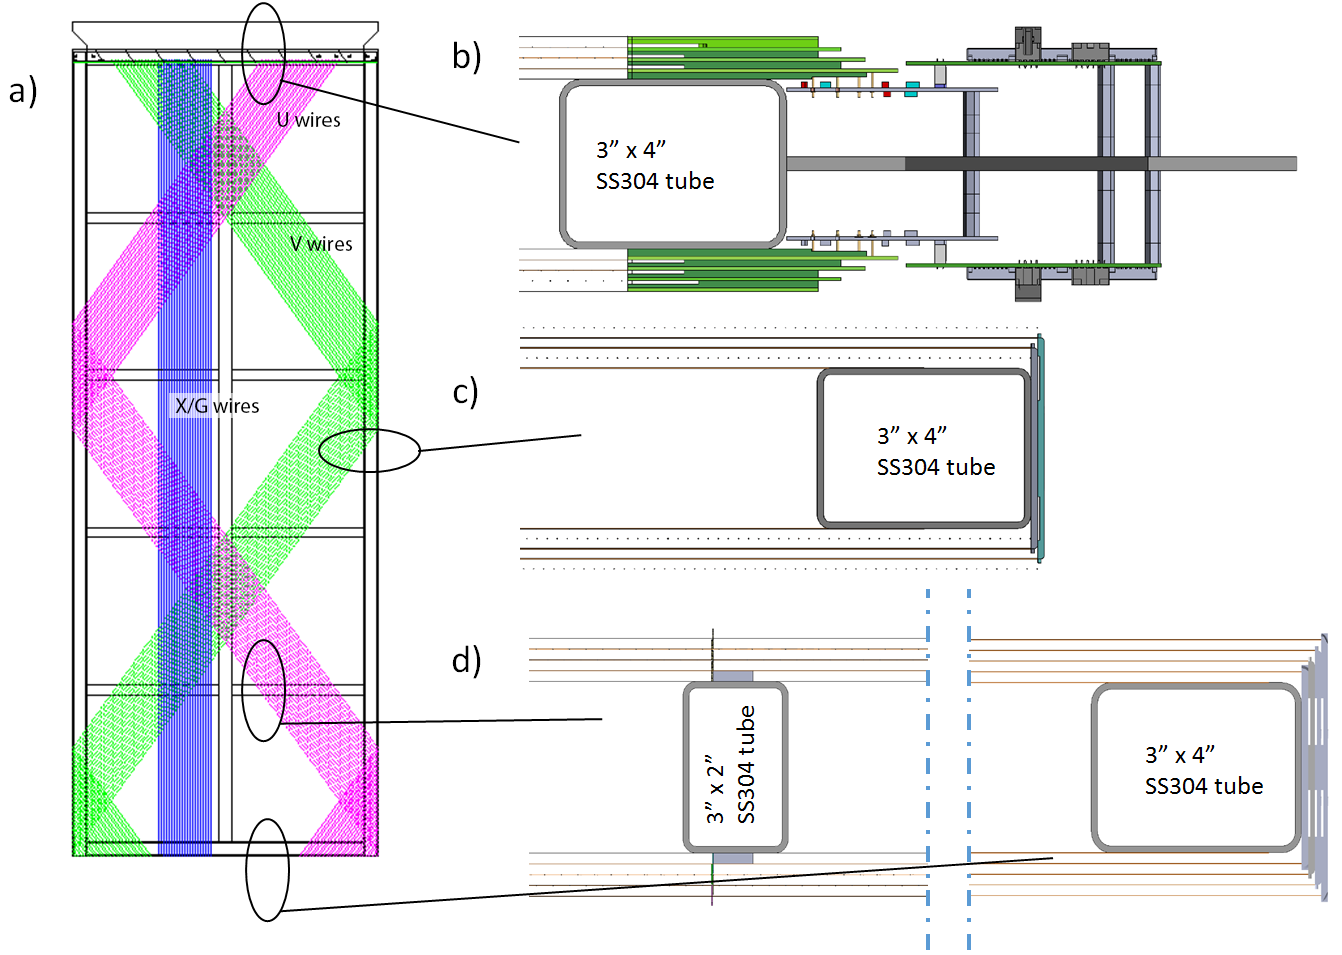
\includegraphics[width=\linewidth]{tpc_apa_cross_sections}
\end{cdrfigure}



%%%%%%%%%%%%%%%%
\subsubsection{APA Frame}
\label{subsec:fd-ref-apaframes}

At a nominal wire tension of 5~N, the total of 3520 wires exert a force of 
$\sim 7.0$~kN/m on the short edges of the APA, and a 
$\sim 1.5 $~kN/m force on the long edges. The wire 
frame must be able to withstand the wire tension with a minimal 
distortion, while minimizing the thickness of the 
frame to reduce the resulting dead space. The wire frame is constructed from all stainless-steel tubes welded in a jig.  
Structural analysis has shown that the maximum distortion of the frame due to wire tension is less than 0.5~mm. The total mass of a bare frame is $\sim$260~kg.

Lengthwise buckling is not an issue, both because of the strength of the frame and because the wires are maintained at an approximately uniform distance from the frame by periodic comb-like structures.

All tube sections are vented to prevent the creation of trapped volumes. The three long tubes have slots cut in them so the photon detectors can be inserted into the APAs after the wires are installed.  The two long outer members of the frame are open-ended, so the photon detector cables can be threaded through them to reach the signal feedthroughs on the cryostat roof.  These long tubes can potentially be used to carry signal and power cables from the bottom APAs cold electronics boards to the signal feedthroughs as well.  Compared with running the middle bottom APA charge readout cables on the floor and then up the wall, this could significantly reduce the cable length for these APAs.


%%%%%%%%%%%%%%%%
\subsubsection{Wire Bonding and Support on an APA}
\label{subsec:fd-ref-wirewrap}


The wire bonding boards physically anchor the wires at the edges of an APA, and also are the interface between the wires and the cold electronics  at the readout end of the APA.  The four planes of wires are attached to their respective wire bonding boards through a combination of epoxy and solder. During winding of the X layer onto the APA the wires are placed across the top surface of the X wire board. The wires are then glued down with a strip of epoxy at the leading edge of the board.  After the epoxy has cured, the wires are soldered onto the copper pads under each wire, and then the wires are cut beyond the pads. The V, U and G planes are attached on top of the X boards and similarly populated with wires, one layer at a time. An array of pins is pushed through holes in the stack of wire bonding boards, making electrical connections between the wires and the capacitor-resistor (or CR) board, which is located between the wire boards and the front end electronics boards.  The CR boards distribute the bias voltages to each wire through current limiting 20~M$\Omega$ resistors,  and bring the charge signal through AC coupling capacitors with sufficient voltage rating to the cold electronics.

These readout boards, as described in Chapter~\ref{sec:detectors-fd-ref-tpc}, generate an estimated $\sim$160 W of heat per APA which may produce a small quantity of argon bubbles.  Stainless-steel covers are placed over the readout boards to contain the bubbles and direct them to the gas volume of the cryostat. This is particularly important for the bottom APAs where the bubbles must be contained and funneled through the vertical hollow frame members to the top of the cryostat to prevent the bubbles entering the TPC's active volume.

Comb like wire support structures (see illustration in the LBNE closeout document) are located on each of the 4 cross beams so that the longitudinal wires are supported every 1.2~m and the angled wires about every 1.5~m while introducing only millimeter-scale dead regions. The support structure is composed of strips of thin G10 sheet, with notches machined at correct intervals.  These wire supports play a key role in minimizing wire deflection due to gravity and electrostatic force, enabling the use of a moderate wire tension and reducing the risk of wire breakage.   They also maintain the correct wire pitch and wire plane separation even if the APA frame has small amount of twist and warp.  If a wire breaks after installation, these intermediate wire support will limit the movement of the broken wire such that it will not travel too far into the drift volume and making contact to the field cage.  To further reduce the risk and impact of a broken wire, we are developing a new wire support scheme that can be applied to the outer wire planes near the bottom of the TPC to keep a broken wire from contact the field cage. 


\begin{cdrfigure}[Winding machine concepts]{tpc-winding-machine}{Illustration of the wire winding machine concept.  The tensioner head is passed from one side of the APA to the other as it is moved around the APA to wind wire onto the APA frame.  The horizontal/vertical positioning systems on each side of the APA are made of commercial linear motion components. }
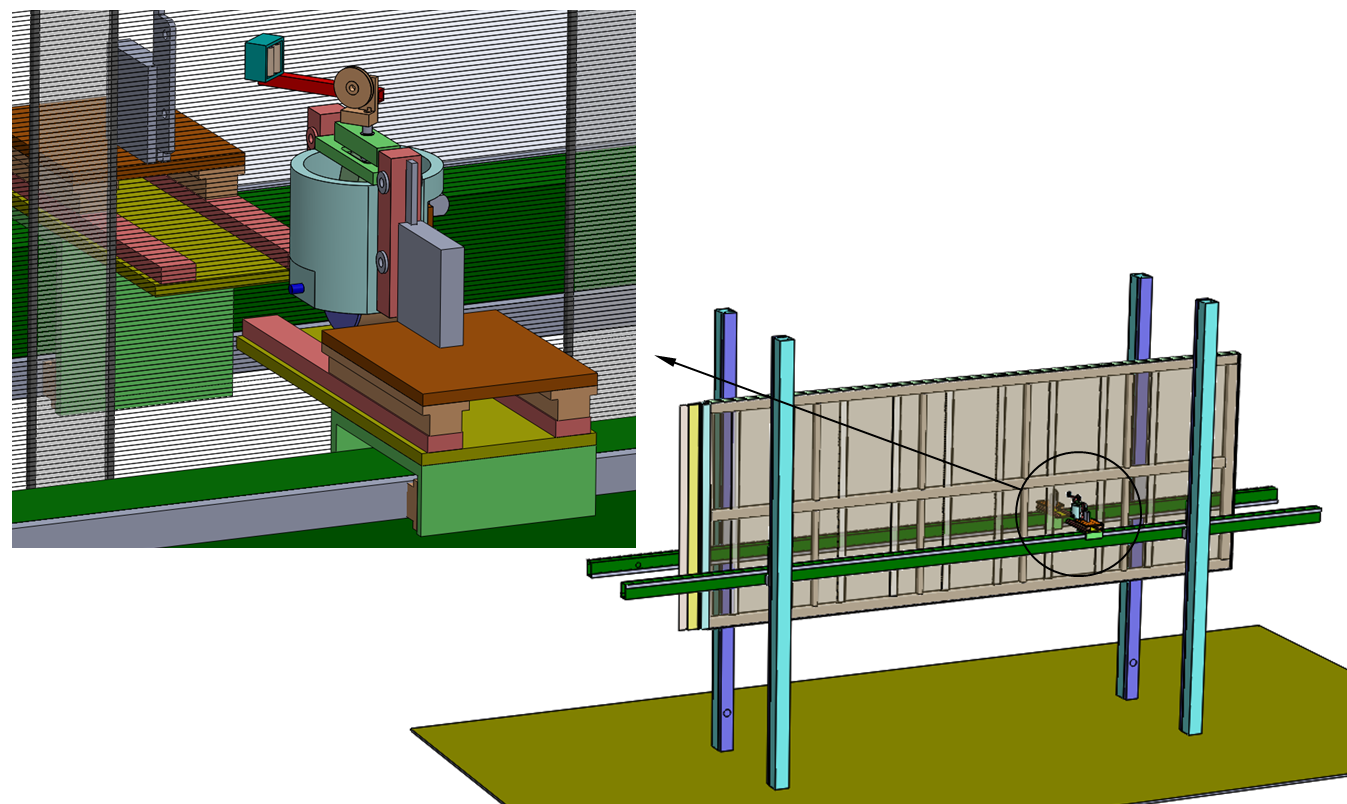
\includegraphics[width=0.9\linewidth]{tpc_apa_winding_machine.png}
\end{cdrfigure}


%%%%%%%%%%%%%%%%
\subsubsection{Wire-Winding Machines}
\label{subsec:fd-ref-wirewinding}

A winding machine will be constructed to lay the 3520 wires onto each APA. It has sufficient versatility that the same mechanism can wind both the angled and the longitudinal layers.  
 
Its working concepts are illustrated in Figure~\ref{fig:tpc-winding-machine}. 
The wire tensioner is a self-contained unit that includes the wire spool.  It is designed so that correct wire tension is maintained independent of the wire feed rate and direction.  The APA is held off the ground by a couple posts, with one of its long edges down.  There are X-Y positioners on either side of the APA; the tensioner is moved across the face of the APA by one of these positioners -- unspooling tensioned wire as it moves.  When the tensioner arrives at the edge of the APA it is passed across to the positioner on the other side of APA while placing the wire into the appropriate slots of the edge boards. In this way the entire layer of wire can be placed on the frame.  

Although a large part of an entire plane of wires can be wound in one continuous process, a more fault-tolerant procedure would be to pause the winding machine periodically and solder the last wire. This intermediate soldering step will prevent the unraveling  of a large section due to an accidental broken wire.  An automatic soldering robot will solder the wire ends after the wires have been laid down on the APA. A wire-tension measuring device will scan the newly placed wires and record the wire tension of each wire. Any wires with abnormal tension will be replaced manually.



%%%%%%%%%%%%%%%%%%%%%%%%%%%%%%%%
\subsection{Cathode Plane Assemblies}
\label{subsec:fd-ref-cpa}

\begin{cdrfigure}[Conceptual design of the cathode plane assembly]{tpc-cathode-model}{Conceptual design of the different cathode plane components near a corner of a cathode wall.  Two flavors of CPAs (outer and inner unit) make up the entire wall of a cathode plane, terminated at both ends by the end pieces (cyan colored).  A high voltage receptacle (orange) connects with the HV feedthrough from the cryostat ceiling. Each CPA is roughly 2.3m wide by 3m tall.}
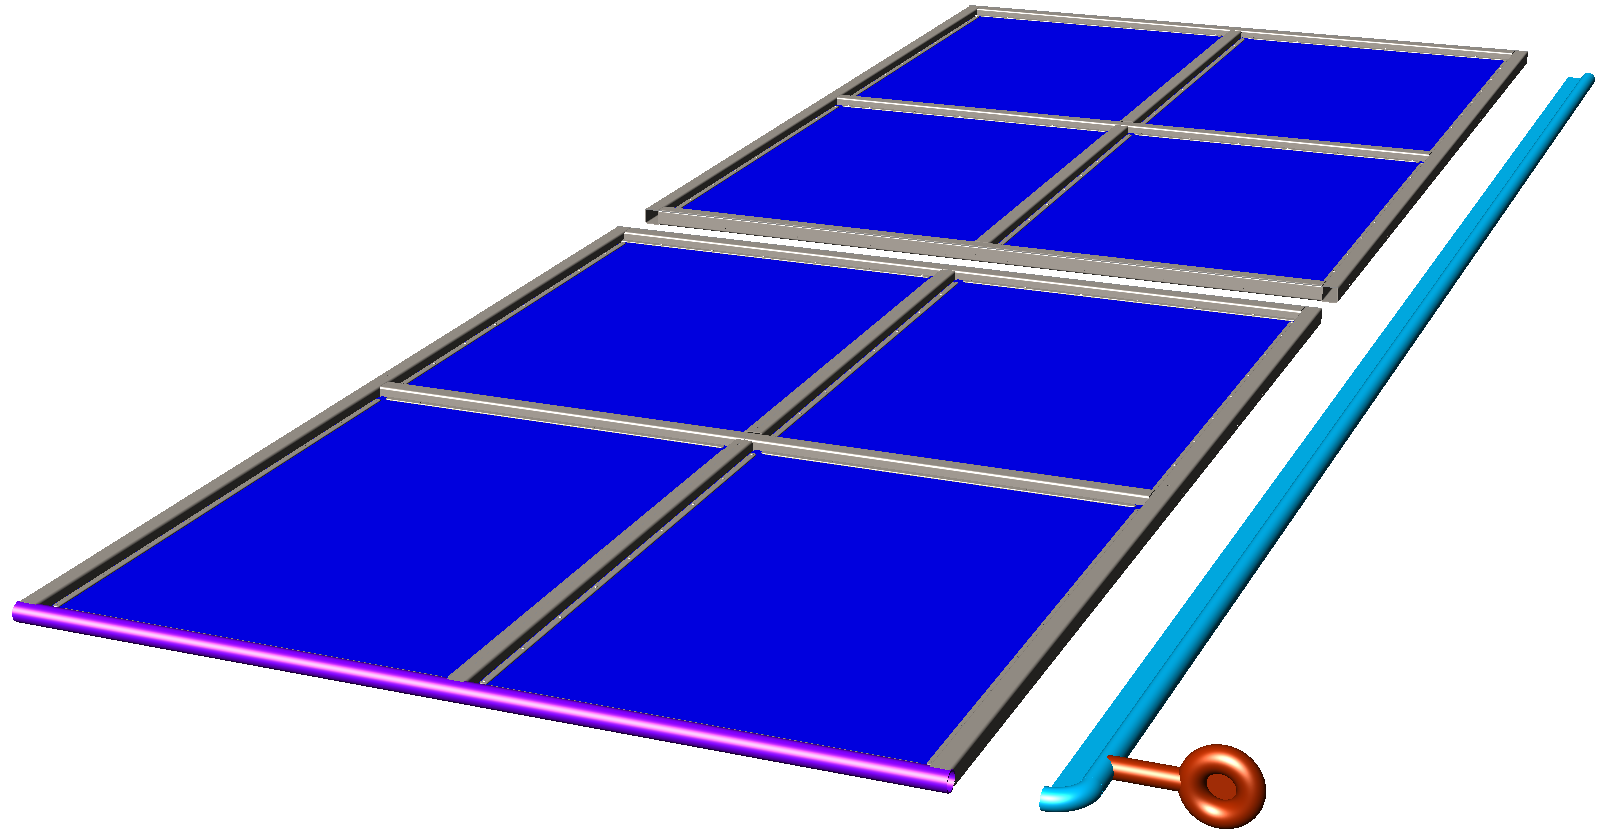
\includegraphics[width=0.9\linewidth]{tpc_cpa_components}
\end{cdrfigure}

There are 2 cathode planes in each detector.  Each plane is tiled from a 4 unit high by 25 unit wide array of cathode plane assemblies (CPAs). Figure~\ref{fig:tpc-cathode-model} shows the building blocks of a cathode plane.  Each CPA is 2.3~m wide (identical to the APA width) and 3~m tall (half of APA height) for ease of fabrication, assembly and handling.  Each CPA is made of a stainless-steel framework, with panels of solid stainless steel sheets mounted between the from openings.  Along each vertical  column of the 4 CPAs, there are two slightly different versions: the outer CPAs (top and bottom rows ), and the inner CPAs (2nd and 3rd rows).  The inner CPAs use all rectangular tubes for the frame structure, while the outer CPAs use 5~cm OD round tubes on the outside edge of the CPA facing the floor or ceiling of the cryostat to minimize the surface electric field.  Two sets of field shaping end pieces are installed at the two ends of a CPA wall to properly terminate the cathode wall with rounded edges.  All CPAs are suspended from the ceiling using G10 hangers under fiberglass rails to insulate the CPAs from the cryostat.

A recent design decision exchanged the positions of the CPAs and APAs in the detector, making the APAs facing the cryostat wall instead of the CPAs as in the LBNE reference design.  This change reduces the stored energy on each cathode plane by about 60\%.  Nevertheless, due to the enormous area of the stainless steel cathode plane, there is still nearly 100~Joules of energy when biased at 180~kV, risking physical damage to the thin membrane structure as well as the CPA structure in the event of a high voltage discharge.  In addition, in such an event, a huge voltage swing could occur on the cathode plane in tens of nanoseconds, injecting a  charge pulse to the sensing wires with a large peak current that could damage the front-end electronics.

To mitigate this risk, we are currently analyze the electrical properties of the cathode, and develop a cathode design that will substantially slowdown the total energy release in case of a discharge.  The best solution appears to be substituting the metallic cathode structure with non-conductive materials with a robust and highly resistive surface coating.  There are many choices of the resistive/anti-static coating material.  We will conduct thorough tests to identify a suitable coating for this application.  Since the electrical current feeding the field cage resistive dividers is supplied through the cathode, it is an interesting challenge to design this high resistive cathode without significant voltage drop along this 58~m long structure.


%%%%%%%%%%%%%%%%%%%%%%%%%%%%%%%%
\subsection{Field Cage}
\label{subsec:fd-ref-fieldcage}

In the TPC, each pair of facing cathode and anode rows forms an electron-drift region. A field cage must completely surround the four open sides of this region
to provide the necessary boundary conditions to ensure a uniform electric field within, unaffected by the presence of the cryostat walls.


\begin{cdrfigure}[35T field cage]{tpc-field-cage}{A corner of the 35ton TPC field cage as it is being constructed}
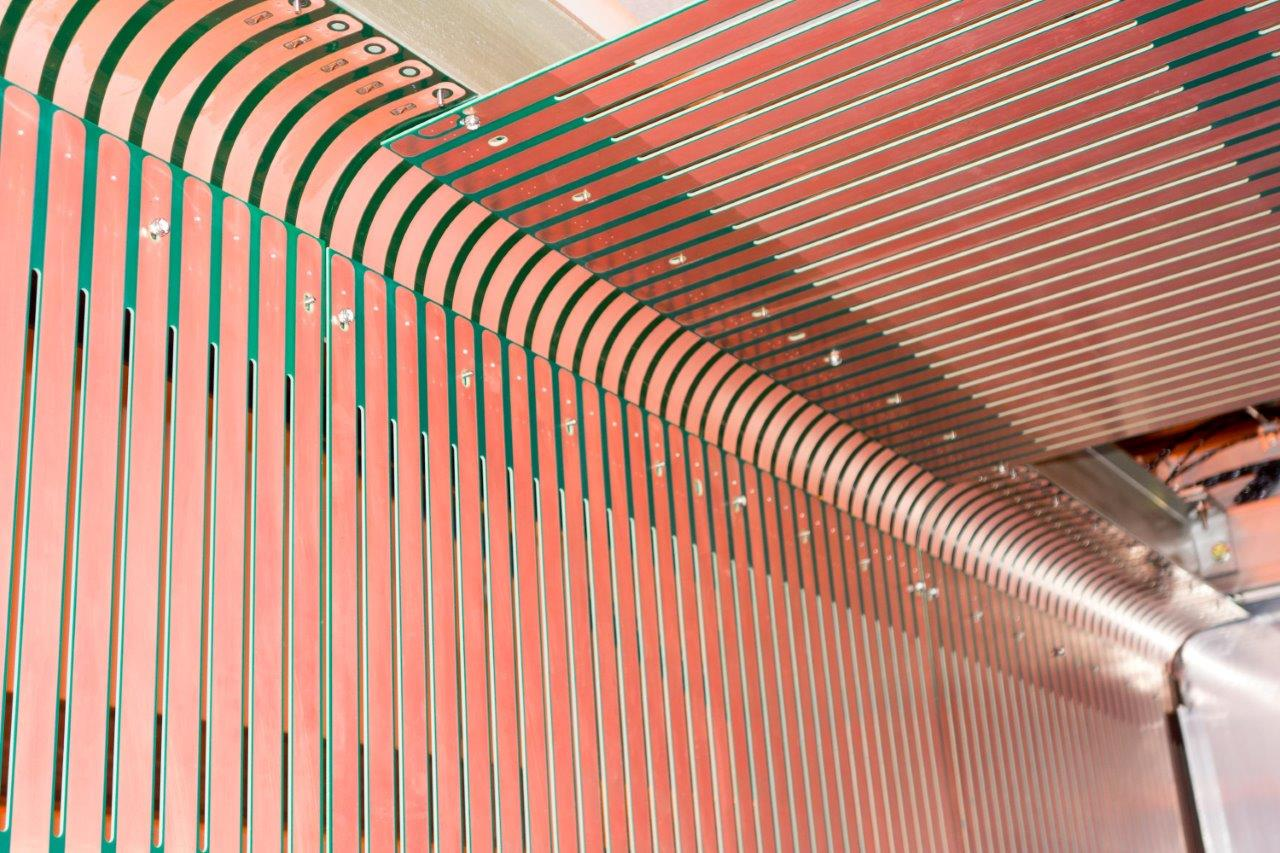
\includegraphics[width=4in]{tpc_fca_35t.jpg}
\end{cdrfigure}


Each 10 kton TPC requires $\sim 2000 \rm{m}^2$ of field 
cage coverage. The field cages are constructed using multiple copper-clad FR4 sheets reinforced with fiber glass I-beams to form modules of 2.3~m $\times$ 3.6~m in size. Parallel copper strips are etched on the FR4 sheets. Strips are biased at appropriate voltages provided by a resistive-divider network. These strips will create a linear electric-potential gradient in the LAr, ensuring a uniform drift field in the TPC's active volume.  Simulations have shown that the drift-field non-uniformity quickly drops to about 1\%, roughly a strip pitch away from the field-cage surface. 

Since the field cage completely encloses the TPC drift region on four sides, while the solid cathodes blocks the remaining two, the field cage sheets must be  perforated to allow liquid argon recirculation in the middle 1/3 of the TPC volume. The ``transparency'' of the perforation will be determined by a detailed LAr computerized fluid dynamic (CFD) study.

The resistor-divider network will be soldered directly onto the field-cage panels. Multiple resistors will be connected in parallel between any two taps of the divider,
in order to provide fault tolerance. One end of the divider chain is connected directly to the cathode, while the other end is connected to ground at the APA through resistors of the appropriate value.  It is envisioned that a pair of field cage modules are pre-attached to the outer CPA modules through hinges, and the field cage modules can be rotated into their final position during installation, or folded back if aisle access is needed (see Figure~\ref{fig:tpc-floor-view}). 
In additional to the resistor network, surge suppressors such as varistors or gas discharge tubes will be installed between each field cage strips to avoid an over-voltage condition occurring between field cage electrodes and the cathode in a high voltage discharge.


The major challenge of this field cage design is to minimize the electric field exposed to the liquid argon near the thin copper strips.  One solution is to cover all copper edges with a thick layer of solder mask (an acrylic based polymer with a high dielectric strength) as part of the standard PCB fabrication steps.  This construction is currently being implemented in the 35ton TPC.  Figure~\ref{fig:tpc-field-cage} shows 
the a section of the partially constructed field cage.  We'll evaluate 35ton TPC test results to determine if this technique is suitable for the much larger far detector. 
 
In the meantime, we are investigating new concepts to minimize the electric field on the field cage.  One example is to apply a very high resistive coating on the outside surface of the field cage such that the surface potential distributes uniformly across the gaps between conductors therefore eliminates the high field region near the conductor edges.  The challenge here is how to ventilate this field cage surface without significantly increasing the field at the perforation.  Another concept is to use roll-formed metal profiles as the field cage electrodes supported by insulating beams.  These profiles have large edge radii that makes their surface electric field relatively low, which makes it possible to be placed closer to the cryostat walls to improve the efficiency in LAr use.  One particular profile is shown in Figure~\ref{fig:tpc-field-cage-roll-form}.  With only a 20~cm distance away from a ground plane, the electric field on the field cage is still under 12~kV/cm.

\begin{cdrfigure}[FCA with roll-formed metal profile]{tpc-field-cage-roll-form}{Left: electrostatic simulation of a field cage design that uses roll-formed metal profiles as the field cage electrodes.  Right: a conceptual design of a field cage module using this profile.}
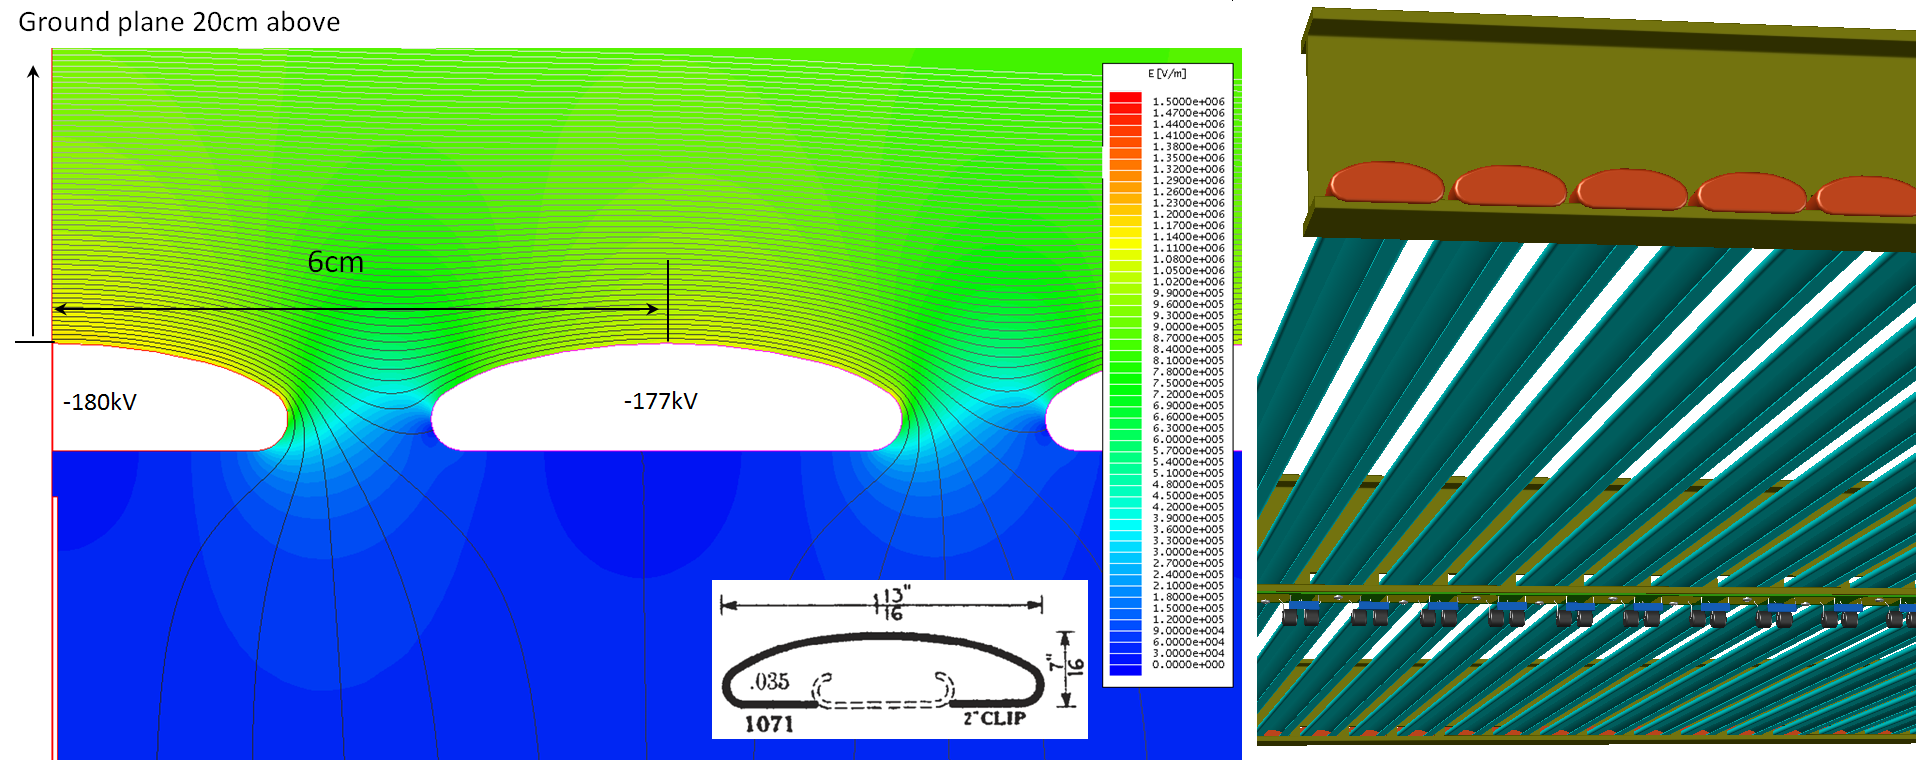
\includegraphics[width=\linewidth]{tpc_fca_rollform.png}
\end{cdrfigure}


%%%%%%%%%%%%%%%%%%%%%%%%%%%%%%%%
\subsection{High Voltage Components}  
\label{subsec:fd-ref-hv}
   
The two cathode planes are biased at $-$180~kV to provide the required 
500~V/cm drift field. Each cathode plane will be powered by a dedicated HV power supply through a RC filter and feedthrough.

The power supplies for the TPC cathode planes must be able to provide $-200$ kV at 1~mA current. The output voltage ripple 
must not introduce more than 10\% of the equivalent thermal noise from the front-end electronics. 
The power supplies must be programmable to trip (shutdown) their output at a certain current limit.  During power on and off, 
including output loss (for any reason), the voltage ramp rate at the feedthrough must be controllable to prevent 
damage to the in-vessel electronics through excess charge injection.  High-voltage feedthroughs must be able to withstand $-$250 kV 
at their center conductors in 1~atm argon gas environment when terminated in liquid argon.

\begin{cdrfigure}[Concept of new feedthrough]{tpc-UCLA-feedthrough}{Top: The high voltage feedthrough and filter developed by the UCLA 
group for the 35ton TPC.  It was tested up to 150 kV.  Bottom: a conceptual design of a new feedthrough for the LAr-FD.}
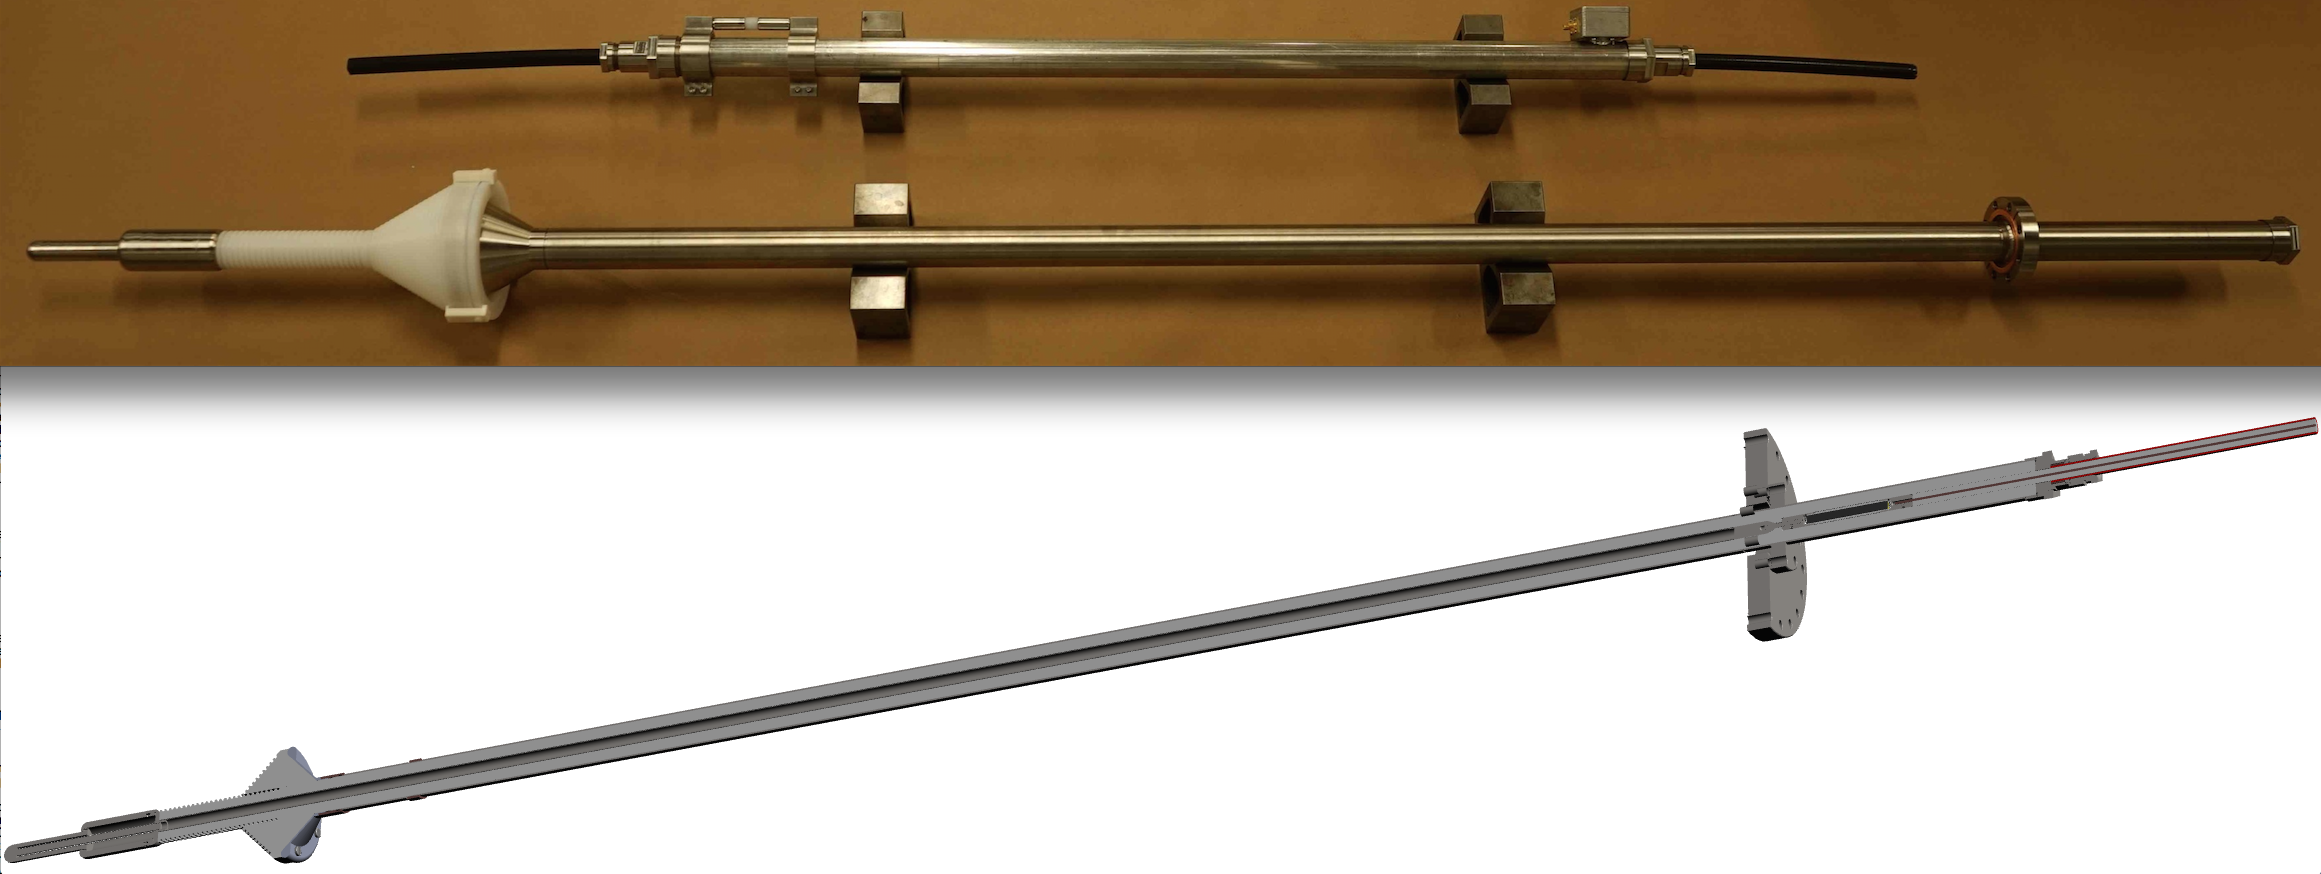
\includegraphics[width=\linewidth]{tpc_hv_feedthrough.png}
\end{cdrfigure}

The current candidate for the high-voltage power supplies is 
the Heinzinger PNC{\it hp} series, which has the lowest output ripple specification.  Additional filtering of the voltage ripples is done through the intrinsic HV cable capacitance and series resistors installed inside the filter box. Established techniques and practices will be implemented to eliminate micro-discharges and minimize unwanted energy transfer in case of an HV breakdown. 
  
To ensure safe and reliable operation, the feedthroughs will be tested at a much higher voltage than expected in
routine operation ($\sim$ 250 kV) in liquid argon. The feedthroughs will be mounted on the ceiling of the cryostat, their cold ends reaching 
through the gas ullage space and submerging into the liquid argon. The center conductor on the cold side of a feedthrough will be 
insulated and shielded by a grounded shroud at least 50~cm below the 
surface of the liquid to ensure bubble free operation at the tip. Figure~\ref{fig:tpc-UCLA-feedthrough} shows an example 
of the feedthrough and filter box made by the UCLA group for the 35ton TPC, as well as the conceptual design of a feedthrough suitable for the LAr-FD TPCs.


%%%%%%%%%%%%%%%%%%%%%%%%%%%%%%%%
\subsection{TPC Prototyping and Test}
\label{subsec:fd-ref-tpc-proto}


Several prototype TPC modules were constructed during the design phase under the LBNE project. The initial prototypes were fractional scale or partial models of the APA and CPA. The CPA prototype was used to evaluate field-shaping electrode attachment techniques. A 40\% scale APA prototype constructed earlier on to study the placement of the wire-wrapping boards and wire-support structures.. It was also used to develop the prototype winding machines. The prototypes were subjected to numerous thermal cycles down to liquid-nitrogen temperature to test the integrity of the wire-to-board and board-to-frame bonds. 

The second set of prototypes are scale models of the APA and CPA. They are being used to validate the designs and to evaluate production procedures. These functional prototypes will be installed in the 35 ton prototype cryostat. This TPC is expected to be operational in 2015.

A TPC prototype that is proposed to go into a CERN test beamline requires 6 full-size APAs with fully instrumented readout electronics, 6 full-size CPAs, and complete field-cage coverage. The TPC will be constructed using identical APAs, CPAs and field-cage panels as designed for the LAr-FD. Additional features will be installed to ensure proper TPC operation given the half-height cryostat configuration. The construction and assembly of all TPC mechanical components will use the same materials and techniques as designed for LAr-FD, with the exception of a reduced degree of automation than will be used to wire APAs for the LAr-FD. 




